\documentclass{beamer}

\beamertemplatenavigationsymbolsempty
\usetheme{Warsaw}

\title{Computer Graphics -- Homework 1}
\author{Tran Phong Binh}
\institute{Student ID: 110062421}
\date{\today}

\begin{document}

\begin{frame}
  \titlepage
\end{frame}

\begin{frame}
  \frametitle{Static Key Controls}
  \begin{itemize}
    \item W: solid/wireframe
    \item Z: previous model
    \item X: next model
    \item O: orthogonal projection
    \item P: perspective projection
    \item I: information output
  \end{itemize}
\end{frame}

\begin{frame}
  \frametitle{Dynamic Key Controls}
  In the modes below, x-, y-, and z-axis are modified according to mouse's horizontal drag, vertical drag, and scrolling, respectively.
  \begin{itemize}
    \item T: model translation
    \item R: model rotation
    \item S: model scaling
    \item E: camera position translation
    \item C: camera center translation
    \item U: camera up translation
  \end{itemize}
\end{frame}

\begin{frame}
  \frametitle{Special Key Control}
  \begin{itemize}
    \item V: model color inversion
  \end{itemize}
  \begin{figure}
    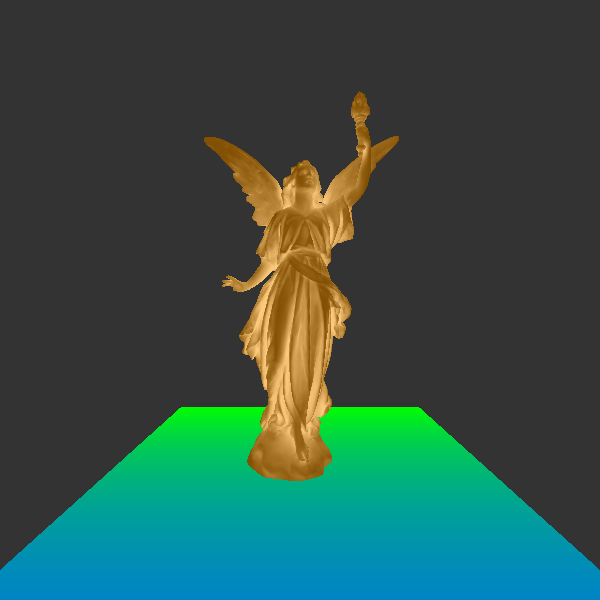
\includegraphics[width=0.5\textwidth]{model_color_inversion}
    \caption{Model color inversion}
  \end{figure}
\end{frame}

\begin{frame}
  \frametitle{Wireframe}
  \begin{figure}
    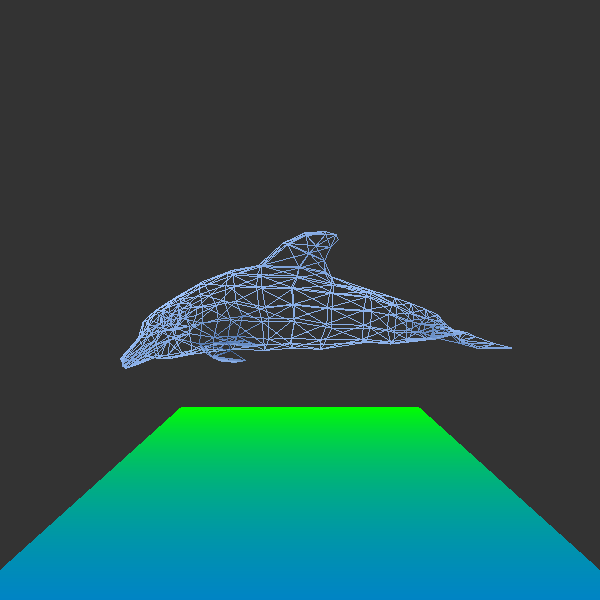
\includegraphics[width=0.5\textwidth]{wireframe}
    \caption{Wireframe}
  \end{figure}
\end{frame}

\begin{frame}
  \frametitle{Orthogonal Projection}
  \begin{figure}
    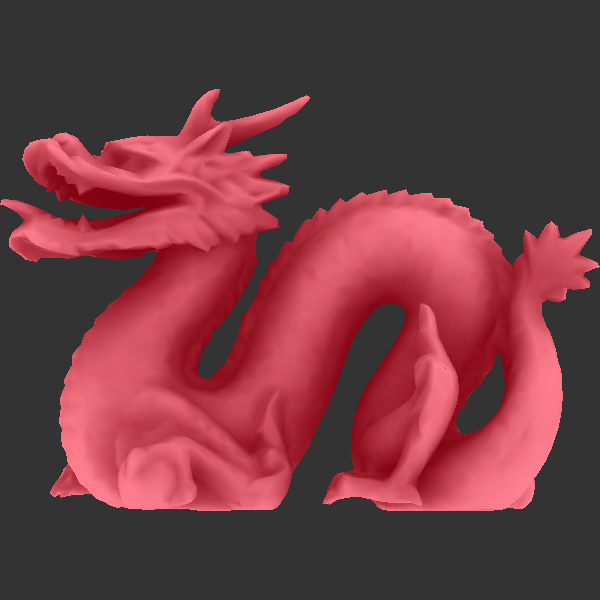
\includegraphics[width=0.5\textwidth]{orthogonal_projection}
    \caption{Orthogonal projection}
  \end{figure}
\end{frame}

\begin{frame}
  \frametitle{Information Output}
  \begin{figure}
    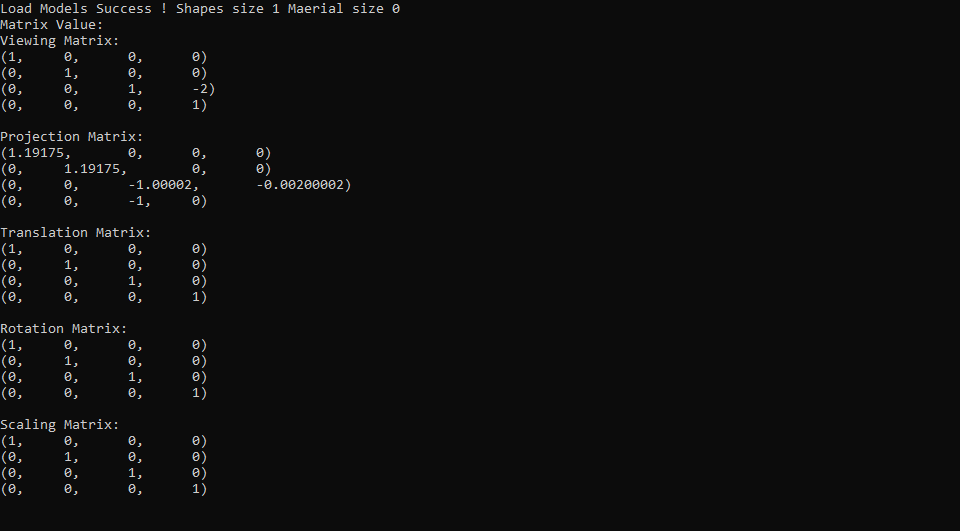
\includegraphics[width=\textwidth]{information_output}
    \caption{Information output}
  \end{figure}
\end{frame}

\begin{frame}
  \frametitle{Aspect Change}
  \begin{figure}
    
\includegraphics[width=0.5\textwidth]{aspect_change}
    \caption{Aspect change}
  \end{figure}
\end{frame}

\begin{frame}
  \frametitle{Model TRS}
  \begin{figure}
    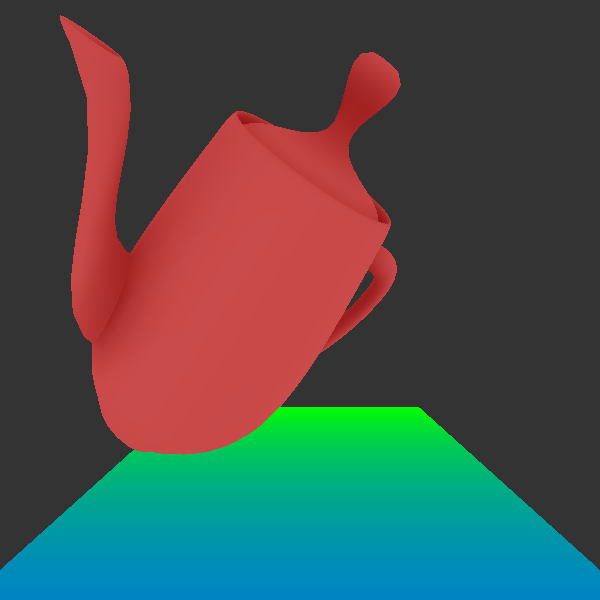
\includegraphics[width=0.5\textwidth]{model_trs}
    \caption{Model translation, rotation, and scaling}
  \end{figure}
\end{frame}

\begin{frame}
  \frametitle{Camera Control}
  \begin{figure}
    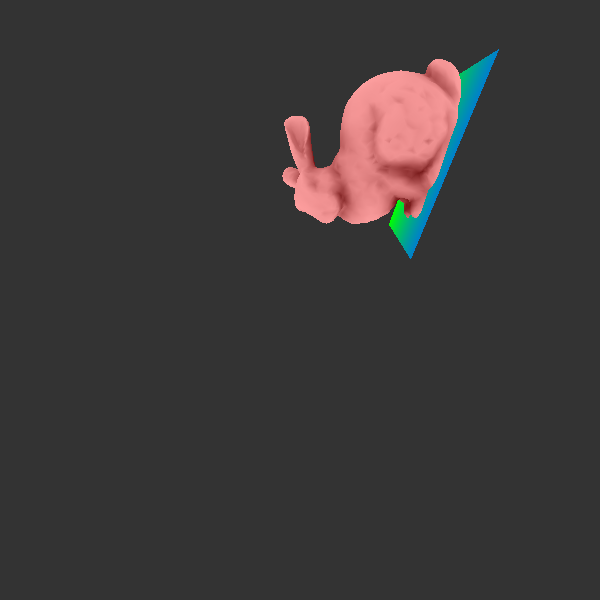
\includegraphics[width=0.5\textwidth]{camera_control}
    \caption{Camera control}
  \end{figure}
\end{frame}

\end{document}
